\section{FileSystem}
    \begin{figure}[h]
        \centering
        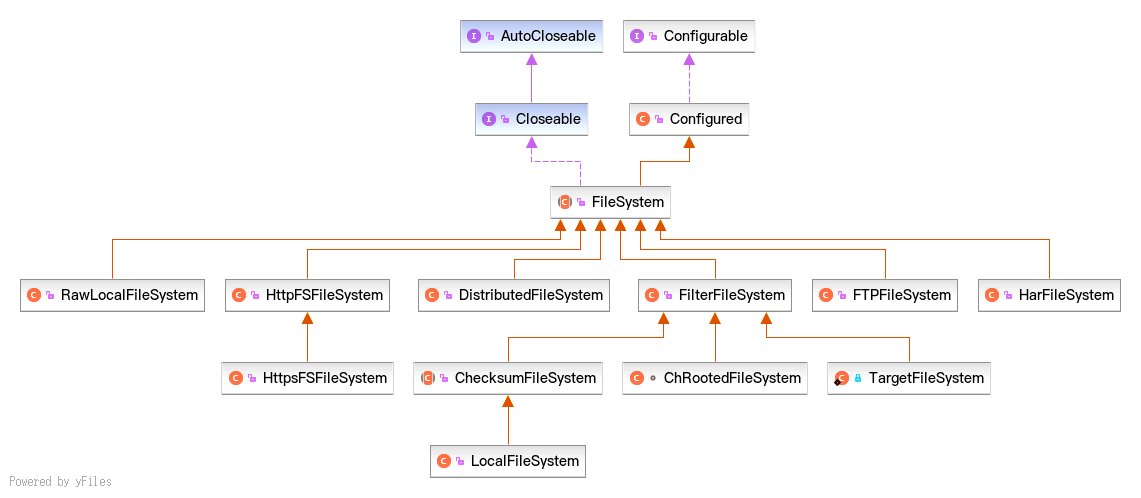
\includegraphics[width=1\linewidth]{filesystemclass}
        \caption{FileSystem 类的 UML 类图}
        \label{fig:filesystemclass}
    \end{figure}
\subsection{}
    \textit{FileSystem}作为文件系统最顶层抽象类,描述了一个文件系统的\textbf{抽象定义},继承了\textit{org.apache.hadoop.conf.Configured}配置基类,并实现了\textit{java.io.Closeable}接口。提供了从XML配置文件生成符合配置描述的文件系统的功能。\\
    \textit{FileSystem}抽象类定义了文件系统所具有的\textbf{基本特征}和\textbf{基本操作}。\textit{FileSystem}具有以下属性:
    \begin{java}[caption=FileSystem attribute]
public static final String FS_DEFAULT_NAME_KEY = 
    CommonConfigurationKeys.FS_DEFAULT_NAME_KEY;
public static final String DEFAULT_FS = 
    CommonConfigurationKeys.FS_DEFAULT_NAME_DEFAULT;

public static final Log LOG = LogFactory.getLog(FileSystem.class);

public static final int SHUTDOWN_HOOK_PRIORITY = 10;

public static final String TRASH_PREFIX = ".Trash";

static final Cache CACHE = new Cache();

private Cache.Key key;

private static final Map<Class<? extends FileSystem>, Statistics> 
    statisticsTable =
        new IdentityHashMap<Class<? extends FileSystem>, Statistics>();

protected Statistics statistics;

private Set<Path> deleteOnExit = new TreeSet<Path>();

    \end{java}
    其中\textit{Cache CACHE}用于缓存已打开的,可缓存的文件系统,启用Cache可以直接\textbf{复用}已打开的文件系统而不必每次都从配置文件生成新的文件系统实例。\\
    \textit{Cache.Key key}所包含的内容就是一个URI的信息及其用户名,作为\textit{Cache}中\textit{Map}的键,与\textit{Cache}一同提供了通过一个合法的URI信息与用户名快速获取到缓存中存在的一个文件系统的对象,从而能够获取到指定文件系统中文件信息的功能。\\
    \textit{statisticsTable} 主要用于保存文件系统的统计信息,作为其\textit{Value}的\textit{Statistics}类使用了\textit{java.util.concurrent.atomic}包中的\textbf{原子变量}属性,提高统计信息的\textbf{一致性},保证\textbf{线程安全}的原子读写操作的同时,提高了\textbf{并行性能}。\\
        \textit{deleteOnExit}作为文件缓存,用来收集当前缓存中的文件\textit{Path}。当文件系统关闭或JVM退出的时候,调用同步方法\textit{processDeleteOnExit}将缓存中的文件全部安全删除。\\
    \\
    \textit{FileSystem}为用户提供了一个访问不同文件系统的统一的\textbf{接口},屏蔽了不同文件系统操作访问上的\textbf{差异性}。其主要提供的方法可以分为两大类:一部分是处理文件和目录相关的事务,另一部分则是文件的读写操作。\\
    以下是\textit{FileSystem}中定义的12个抽象方法,这12个方法应该是一个文件系统应具有的\textbf{基本操作},可归纳为获取文件系统URI,打开文件,创建文件,追加文件,重命名文件,删除文件,获取文件列表,获取和设置工作目录,创建文件夹,获取文件状态。其具体的实现则是取决于不同的文件系统的特点。
    \begin{java}[caption=FileSystem abstract method]
public abstract URI getUri();

public abstract FSDataInputStream open(Path f, int bufferSize) throws IOException;

public abstract FSDataOutputStream create(Path f,
    FsPermission permission,
    boolean overwrite,
    int bufferSize,
    short replication,
    long blockSize,
    Progressable progress) throws IOException;

public abstract FSDataOutputStream append(Path f, int bufferSize, Progressable progress) throws IOException;

public abstract boolean rename(Path src, Path dst) throws IOException;

public abstract boolean delete(Path f) throws IOException;

public abstract boolean delete(Path f, boolean recursive) throws IOException;

public abstract FileStatus[] listStatus(Path f) throws IOException;

public abstract void setWorkingDirectory(Path new_dir);

public abstract Path getWorkingDirectory();

public abstract boolean mkdirs(Path f, FsPermission permission) throws IOException;

public abstract FileStatus getFileStatus(Path f) throws IOException;

    \end{java}

\subsection{基于FileSystem实现的文件系统概述}
    \subsubsection{RawLocalFileSystem}
        \textit{RawLocalFileSystem}是\textit{Hadoop}中实现的本地文件系统,在该类中与文件元数据和目录相关的操作,都是通过\textbf{装饰器模式}适配到\textit{java.io.File}的对应API来完成的。\\
        \textit{LocalFSFileInputStream}的构造函数如下:
        \begin{java}[caption=LocalFSFileInputStream]
class LocalFSFileInputStream extends FSInputStream {
    public LocalFSFileInputStream(Path f) throws IOException {
        this.fis = new TrackingFileInputStream(pathToFile(f));
    }
}
        \end{java}
        \begin{java}[caption=TrackingFileInputStream]
class TrackingFileInputStream extends FileInputStream {
    public TrackingFileInputStream(File f) throws IOException {
        super(f);
    }
}
        \end{java}
    可以看出,\textit{LocalFSFileInputStream}中包装了\textit{TrackingFileInputStream},而\textit{TrackingFileInputStream}则是包装了\textit{FileInputStream}。

    \subsubsection{FilterFileSystem}
        \textit{FilterFileSystem}类主要是在其内部定义了一个\textit{Filesystem}属性用于包含其他文件系统,\textit{FilterFileSystem}用作其基本文件系统,\textbf{可能性}的提供转换数据或附加功能。\\
        \textit{FilterFileSystem}类本身简单地覆盖\textit{FileSystem}的所有方法,将所有请求传递给其包含的文件系统\textit{fs}。
        \begin{java}[caption=FilterFileSystem]
public class FilterFileSystem extends FileSystem {
    protected FileSystem fs;
    @Override
    public void concat(Path f, Path[] psrcs) throws IOException {
        fs.concat(f, psrcs);
    }
}
        \end{java}

    \subsubsection{ChecksumFileSystem}
        \textit{ChecksumFileSystem}类是一个基于校验和的文件系统的抽象类,它继承自\textit{FilterFileSystem}类,其特点就是在客户端为每一个原生文件(raw file)创建一个扩展名为\textbf{“.crc”}的校验和文件,用来校验原生文件的完整性。
        \begin{java}[caption=ChecksumFileSystem]
private int bytesPerChecksum = 512; 
private boolean verifyChecksum = true; 
        \end{java}
        
        \textit{ChecksumFSInputChecker}用于在写入过程中根据配置生成其校验和文件,\textit{ChecksumFSOutputSummer}用于读取过程中依据校验文件对原生文件进行正确性校验。
        \begin{itemize}
            \item[*] org.apache.hadoop.fs.ChecksumFileSystem.ChecksumFSInputChecker      
            \item[*] org.apache.hadoop.fs.ChecksumFileSystem.ChecksumFSOutputSummer
        \end{itemize}

    \subsubsection{LocalFileSystem}
        \textit{LocalFileSystem}类实现了\textit{FileSystem}的API,它是一个基于\textbf{校验和}的本地文件系统。\\
        它是以\textit{RawLocalFileSystem}为基本文件系统。
        \begin{java}[caption=LocalFileSystem]
public LocalFileSystem() {  
    this(new RawLocalFileSystem());  
}  
public LocalFileSystem(FileSystem rawLocalFileSystem) {  
    super(rawLocalFileSystem);  
    rfs = rawLocalFileSystem;  
} 
        \end{java}
        
        \textit{reportChecksumFailure}方法实现了向文件系统\textbf{报告}校验和文件出错,同时把出错的校验和文件重命名后,移动到指定的\textit{bad\_files}目录中,在该目录中的文件是\textbf{不能}够被重新使用的。\\
        \begin{java}[caption=reportChecksumFailure]
public boolean reportChecksumFailure(Path p, FSDataInputStream in, long inPos, FSDataInputStream sums, long sumsPos) {
    try {
        File f = ((RawLocalFileSystem)fs).pathToFile(p).getCanonicalFile();
        String device = new DF(f, getConf()).getMount();
        File parent = f.getParentFile();
        File dir = null;
        while (parent != null && FileUtil.canWrite(parent) && parent.toString().startsWith(device)) {
            dir = parent;
            parent = parent.getParentFile();
        }

        if (dir==null) {
            throw new IOException("not able to find the highest writable parent dir");
        }
            
        File badDir = new File(dir, "bad_files");
        if (!badDir.mkdirs()) {
            if (!badDir.isDirectory()) {
            throw new IOException("Mkdirs failed to create " + badDir.toString());
            }
        }
        String suffix = "." + rand.nextInt();
        File badFile = new File(badDir, f.getName()+suffix);
        LOG.warn("Moving bad file " + f + " to " + badFile);
        in.close();                               // close it first
        boolean b = f.renameTo(badFile);                      // rename it
        if (!b) {
            LOG.warn("Ignoring failure of renameTo");
        }

        File checkFile = ((RawLocalFileSystem)fs).pathToFile(getChecksumFile(p));
        sums.close();
        b = checkFile.renameTo(new File(badDir, checkFile.getName()+suffix));
        if (!b) {
            LOG.warn("Ignoring failure of renameTo");
            }
    } catch (IOException e) {
        LOG.warn("Error moving bad file " + p + ": " + e);
    }
    return false;
}
        \end{java}

    \subsubsection{DistributedFileSystem}
        对\textit{HDFS}的用户来说,\textit{DistributedFileSystem}就代表了\textit{Hadoop}\textbf{分布式}文件系统,用户只要操作\textit{DistributedFileSystem}的对象来进行文件目录的建立、数据的存取操作,其他的都由\textit{DistributedFileSystem}来完成,所以它为我们提供了一个\textit{HDFS}的用户界面。
        \begin{java}[caption=DistributedFileSystem]
public class DistributedFileSystem extends FileSystem {  
    private Path workingDir;  
    private URI uri;  
    DFSClient dfs;  
    private boolean verifyChecksum = true;  
        
    static{  
        Configuration.addDefaultResource("hdfs-default.xml");  
        Configuration.addDefaultResource("hdfs-site.xml");  
    }  
    
    public DistributedFileSystem() {  
    }  
}  
        \end{java}

        但是在\textit{HDFS}内部,通过\textbf{适配器模式}将真正的操作步骤是交给了与服务器端交互的\textit{HDFS}客户端\textit{DFSClient}去完成,实现与\textit{HDFS}集群上的其他节点进行交互功能。\\
        例如\textit{HDFS}的\textit{rename}方法实际上是适配到了\textit{DFSClient}的\textit{rename}方法。
        \begin{java}[caption=DistributedFileSystem.rename]
public void rename(Path src, Path dst, final Options.Rename... options) throws IOException {
    statistics.incrementWriteOps(1);
    storageStatistics.incrementOpCounter(OpType.RENAME);
    final Path absSrc = fixRelativePart(src);
    final Path absDst = fixRelativePart(dst);
    try {
        dfs.rename(getPathName(absSrc), getPathName(absDst), options);
    } catch (UnresolvedLinkException e) {
        final Path source = getFileLinkStatus(absSrc).getPath();
        new FileSystemLinkResolver<Void>() {
            @Override
            public Void doCall(final Path p) throws IOException {
                dfs.rename(getPathName(source), getPathName(p), options);
                return null;
            }
            @Override
            public Void next(final FileSystem fs, final Path p) throws IOException {
                return doCall(p);
            }
        }.resolve(this, absDst);
    }
}
        \end{java}
        用户调用\textit{DFSClient}的一个写入方法,\textit{DFSClient}返回给用户一个输入流,用户向输入流中写入数据,写入的数据被\textbf{透明的重定向}到一个本地临时文件中,当写入数据量达到一个块容量(默认64M)或写入正常结束时,\textit{DFSClient}向\textit{NameNode}发送请求,\textit{NameNode}回应一个\textit{DataNode}列表。\textit{DFSClient}将本地临时文件的数据传输到\textit{DataNode1}上,\textit{DataNode1}以4K为单位逐步接收数据,储存在本地仓库的同时将数据传输给\textit{DataNode2},\textit{DataNode2}与\textit{DataNode1}行为相同,像\textbf{管道流水}一样将数据传输到\textit{DataNode3},\textit{DataNode3}只储存数据。\\
        当用户输入正常结束时,\textit{NameNode}将操作\textbf{追加}到日志并\textbf{储存},文件写入正式生效。如果输入意外中断失败,则储存的文件丢失。\\
        在默认配置下,会有三个内容相同的\textit{DataNode}互为\textbf{备份冗余}以保证数据的\textbf{可靠性}。其中,\textit{DataNode1}和\textit{DataNode2}位于同一机架的不同节点上,数据传输代价较低,但同时损毁的可能性也较大。\textit{DataNode3}则位于不同机架上,传输数据代价大,但更为安全可靠。\\
        \textit{Hadoop}采用这种\textit{DataNode}分布策略在数据备份\textbf{可靠性}和性能\textbf{延时}上做出了平衡。
        \begin{figure}[h]
            \centering
            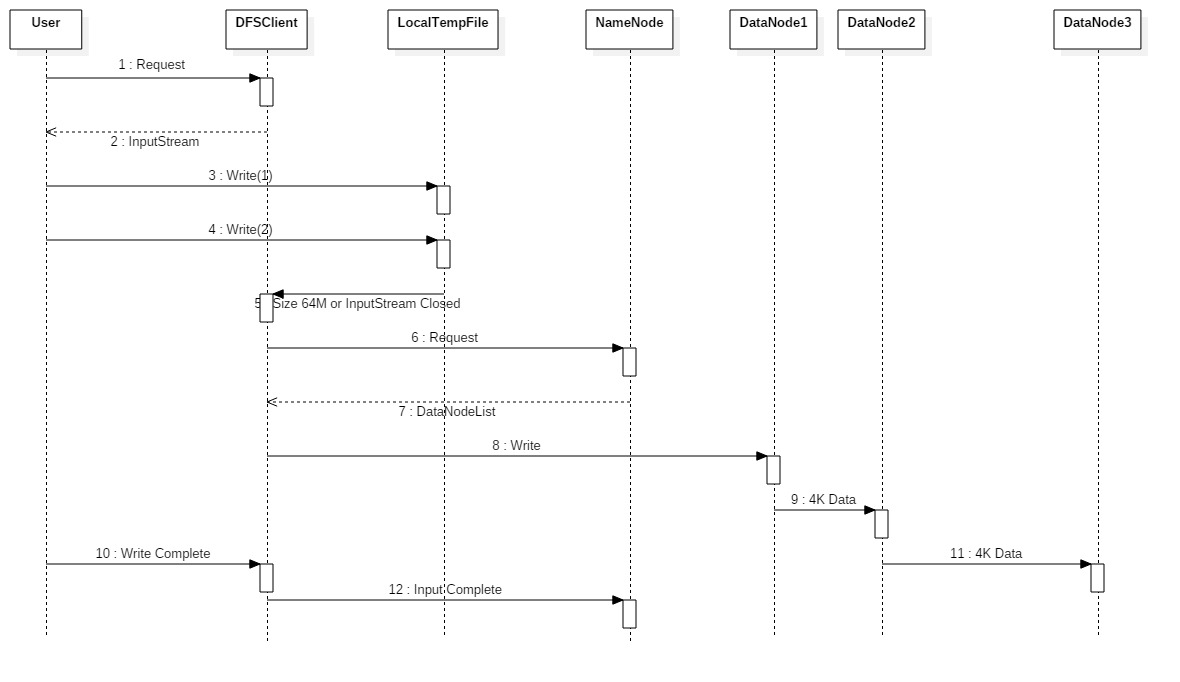
\includegraphics[width=1\linewidth]{HDFSInputTime}
            \caption{一个简单的HDFS写入操作时序图}
            \label{fig:HDFS Input Time}
        \end{figure}


    \subsubsection{其他文件系统实现}
        \begin{itemize}
            \item[*] HarFileSystem:归档文件系统
            \item[*] HttpFSFileSystem:基于Http协议的网络文件系统
            \item[*] HttpsFSFileSystem:基于Https协议的网络文件系统
            \item[*] FTPFileSystem:基于FTP文件传输协议的文件系统
        \end{itemize}


%% 结束
\endinput